% Created 2020-10-02 Fri 11:29
% Intended LaTeX compiler: pdflatex
\documentclass[11pt]{article}
\usepackage[utf8]{inputenc}
\usepackage[T1]{fontenc}
\usepackage{graphicx}
\usepackage{grffile}
\usepackage{longtable}
\usepackage{wrapfig}
\usepackage{rotating}
\usepackage[normalem]{ulem}
\usepackage{amsmath}
\usepackage{textcomp}
\usepackage{amssymb}
\usepackage{capt-of}
\usepackage{hyperref}
\usepackage {ctex}
\author{lin chuan}
\date{\today}
\title{}
\hypersetup{
 pdfauthor={lin chuan},
 pdftitle={},
 pdfkeywords={},
 pdfsubject={},
 pdfcreator={Emacs 26.3 (Org mode 9.3.8)}, 
 pdflang={English}}
\begin{document}

\tableofcontents

\section{简答题}
\label{sec:org67a7e40}
\subsection{分苹果}
\label{sec:org15c51dc}

一共2000个苹果,有任意多个箱子用来装苹果,要求一个或多个箱子中的苹果数量之和可以得到1到2000中的任意数目的苹果。

请问最少需要多少个箱子才能满足上述条件?
\subsection{地址问题}
\label{sec:org9a25ce6}

某计算机内存为64MB, 字长为4字节, 请问其地址总线的取值范围

\section{下面代码段的输出是什么, 并给出解释}
\label{sec:orgc2576ef}

\begin{verbatim}
let p = []; 
let s = "string"; 
let i; 
for (i = 0; i < s.length; i++) 
     p[i] = s[length - i]; 
console.log(p.join(""));
\end{verbatim}

\begin{itemize}
\item a) gnirts
\item b) gnirt
\item c) string
\item d) 没有输出
\end{itemize}

\section{下面程序段输出什么, 并给出解释}
\label{sec:org0946ef5}
\begin{verbatim}
let n = 0, m = 0;
if (n > 0) {
    if (m > 0) {
	console.log("True");
    }
    else {
	console.log("False");
    }
}
\end{verbatim}

\begin{itemize}
\item a) True
\item b) False
\item c) 没有输出
\item d) 运行错误
\end{itemize}

\section{二叉树如下,使用先序遍历的结果是:}
\label{sec:org32bbe59}
\begin{center}
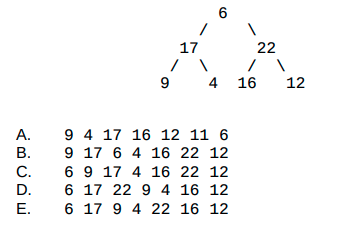
\includegraphics[width=.9\linewidth]{./img/1234.png}
\end{center}

\section{二叉搜索树如下, 请问以何种顺序输入无法构造这样的二叉树}
\label{sec:orgc721137}

\begin{center}
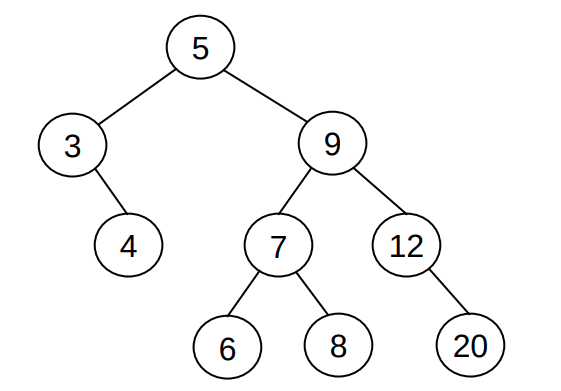
\includegraphics[width=.9\linewidth]{./img/111222.png}
\end{center}

\begin{center}
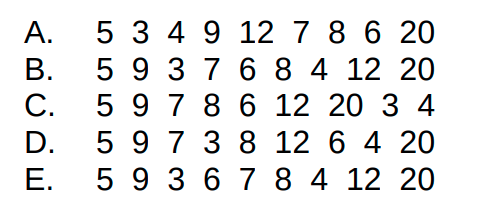
\includegraphics[width=.9\linewidth]{./img/111223.png}
\end{center}

\section{将如下输入转换为最大堆}
\label{sec:org0c348ce}

\begin{verbatim}
{1, 2, 8, 10, 20, 6, 16, 14, 31, 7}
\end{verbatim}

\textbf{提示}:  结果应当是唯一的; 你可以使用数组或是画图作为答案.

\section{将如下输入转换为最小堆}
\label{sec:org39af9ca}

\begin{verbatim}
{1, 2, 8, 10, 20, 6, 16, 14, 31, 7}
\end{verbatim}

\textbf{提示}:  结果应当是唯一的; 你可以使用数组或是画图作为答案.
\section{使用直线划分空间}
\label{sec:orgba43e2d}

如下图所示:

\begin{center}
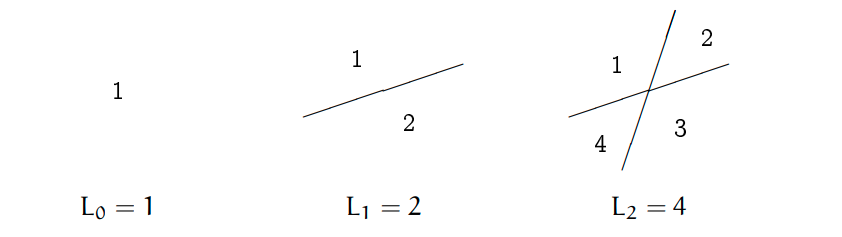
\includegraphics[width=.9\linewidth]{img/line.png}
\end{center}

\begin{itemize}
\item 0根直线可以划分出1个空间
\item 1根直线可以划分出2个空间
\item 2根直线可以划分出4个空间
\end{itemize}

\textbf{问题}:

\begin{enumerate}
\item 写出公式L(n); n表示折线数量, L(n)表示通过n根折线可以划分出的最多的空间数量
\item 使用js语言实现计算L(n)的函数
\begin{verbatim}
function calc_line_spaces(n); // n >= 0
\end{verbatim}
\end{enumerate}

\section{使用折线划分空间}
\label{sec:org3c23450}

如下图所示:
\begin{itemize}
\item 0根折线可以划分出1个空间
\item 1根折线线可以划分出2个空间
\item 2根折线最多可以划分出7个空间
\end{itemize}

\begin{center}
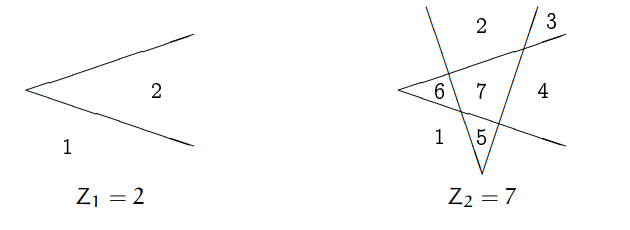
\includegraphics[width=.9\linewidth]{./img/zline.png}
\end{center}


\textbf{问题}:

\begin{enumerate}
\item 写出公式Z(n); n表示折线数量, Z(n)表示通过n根折线可以划分出的最多的空间数量
\item 使用js语言实现计算Z(n)的函数
\begin{verbatim}
function calc_zig_spaces(n); // n >= 0
\end{verbatim}
\end{enumerate}

\section{打印三角形}
\label{sec:orgf183a24}
\begin{center}
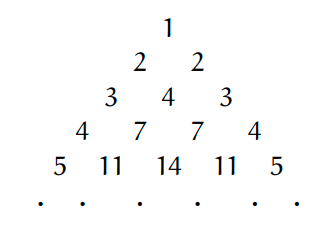
\includegraphics[width=.9\linewidth]{./img/triangle.png}
\end{center}

观察上图三角形的规律,实现函数根据输入n打印n行如图所示三角形.
\begin{verbatim}
fuction draw(n); // n > 0
\end{verbatim}

\section{实现atof函数}
\label{sec:org4eb1669}
\begin{itemize}
\item 函数定义
\begin{verbatim}
function my_atof(str);
\end{verbatim}
\item 函数描述

\texttt{my\_atof()} 会扫描参数str字符串,跳过前面的空格字符,直到遇上数字或 \texttt{.} 符号才开始做转换,而遇到非数字或字符串结束时才结束转换,并将结果返回。

以下都是合法输入:
\begin{verbatim}
0.123z
.123k
16.4cc
16.
0.0
0.
\end{verbatim}

\begin{verbatim}
注意: 
  1. 不考虑 +- 符号, 不考虑输入非法的情况 
  2. 使用Number()构造函数无法实现这个功能
     例如: Number(".32b")
	   NaN
\end{verbatim}
\end{itemize}

\section{使用栈的数据结构实现队列的功能}
\label{sec:org4bc231e}

js的数组已经提供了push和pop的方法, 也提供了length属性.

请使用已有的栈的方法(push, pop)和属性(length)实现一个队列的功能:

要求: 只能使用push和pop以及length, 不能使用其他方法和属性.

请补全下列代码, 要求运行后能输出从1到9

\begin{verbatim}
class Queue{
    constructor() {
	this.data = [];
	this.length = 0;
    }

    enqueue(item) {
	// your code
    }

    dequeue() {
	// your code
    }

    isEmpty() {
	// your code
    }
}

let q = new Queue();
for(let i = 1; i < 10; i++) {
    q.enqueue(i);
}

while(!isEmpty(q)) {
    console.log(q.dequeue());
}
\end{verbatim}

\section{彩票生成器}
\label{sec:org42622c9}
\texttt{从红色球号码(1-33)中选择6个号码,从蓝色球号码(1-16)中选择1个号码,组合为一注号码。}

请你根据上述规则实现程序, 生成一个彩票的号码.
\end{document}
